
\subsection{Creación de Planimetría}

% A- Módulo de planimetría
% - Objetivo del módulo	
El objetivo de este módulo es caracterizar el escenario donde transcurre el movimiento. Actualmente las trayectorias en Navindoor, se centran en el movimiento en interiores, por lo que se ofrece las heramientas básicas para caracterizar un edifício de varias plantas. Esta carazterización nos proveerá información sobre las restricciones de movimiento, posición de puntos de acceso, altura, etc. Esta información puede ser usada por los modelos simulación de trayectorias, señales, además de los algoritmos de localización.
% - Modelización 
%     - Diagrama de clases
%     - nodos, paredes, puertas, ascensores, escaleras, APs, plantas

Con este fin se ha definido clases de MATLAB que representarán los distintos objetos necesarios para la caracterización de un edificio. Se ha creado la clase \emph{node}, para representar un punto en el espacio tridimensional, a partir de este objeto se construyen las demás clases. Los objetos que representa las paredes del edifício, son construidos a partir de dos objetos \emph{node}. Existen tambien elementos que tiene una posición puntual, por lo que se ha creado clases que heredan las propiedades de \emph{node}. Estos son objetos \emph{stairs}, \emph{elevators}, \emph{doors}, \emph{beacons}. Los dos primeros nos idican los puntos de escape de una planta. Los objetos \emph{doors}, se definen dentro de los objetos \emph{wall}s, y permiten el paso en su entorno. Por último los objetos \emph{beacons}, representan puntos de acceso generadores de señales de radio frecuencia. Estos elementos son encapsulados en la clase \emph{level}, de modo que los objetos antes mencionados son atributos de los objetos \emph{level}. Por último se ha creado un clase, llamado \emph{building}, que en sus atributos contiene un lista de objetos \emph{levels}. Este esquema de clases se muestra en la figura \ref{fig:esquemabuilding}.

\begin{figure}[!ht]
    \centering
    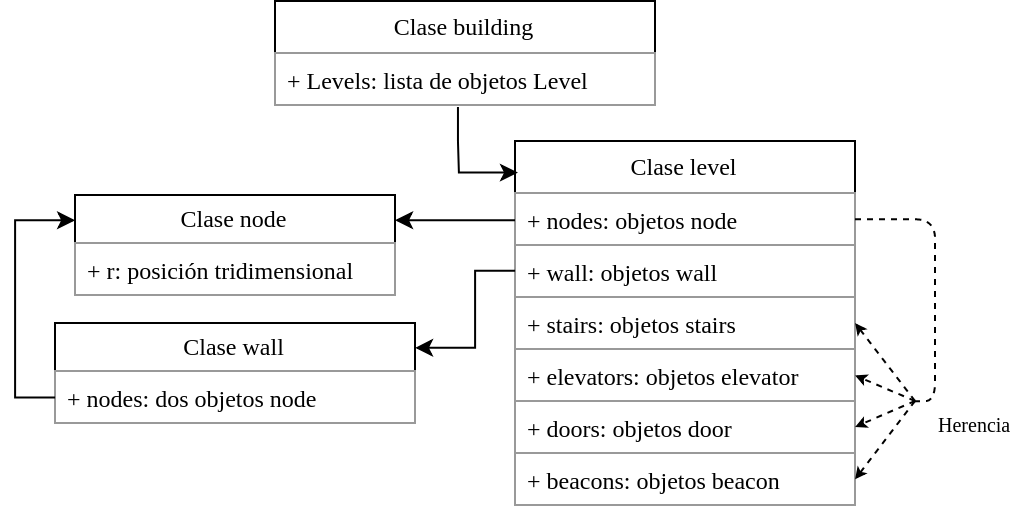
\includegraphics[width=1.05     \columnwidth]{img/Design/planimetria.png} 
    \caption[]{Esquema de la clases }
    \footnotesize
    En la imagen se intenta mostra 
    \label{fig:esquemabuilding}
\end{figure}  


% - Explicación básica del proceso de generación de planimetría:  
%     - Clicks con el ratón 
%     - mapa real como plantilla
%     - Visualización 3D
Para la creación de cada uno de estos objetos existe un constructor siguiendo las bases de la programación orientada a objetos, sin embargo la carazterización del escenario de esta forma puede ser muy tediosa. Es por ello que se ha optado en el desarrollo de una interfaz gráfica (figura \ref{fig:interfaz1}), que nos ayude en este trabajo. De esta forma se puede definir objetos \emph{nodes} con simples \emph{clicks}, y paredes uniendo objectos \emph{nodes}. 
Debido a que el proceso de creación de la planimetría puede ser tedioso, navindoor contiene una GUI capaz de generar un objeto \emph{building} (figura \ref{fig:interfaz1}). La interfaz nos permite crear los objetos antes mencionados con unos simples \emph{clicks}, además de permitir cargar una imagen de los planos reales con la que ayudarnos a construir la planimetría. Ademaś, cabe mencionar que la GUI contiene herramientas necesarias para la visualización en 3D, la modificación y eliminación de los elementos, haciendo la construcción de la planimetría intuitiva.

\begin{figure}
    \centering
    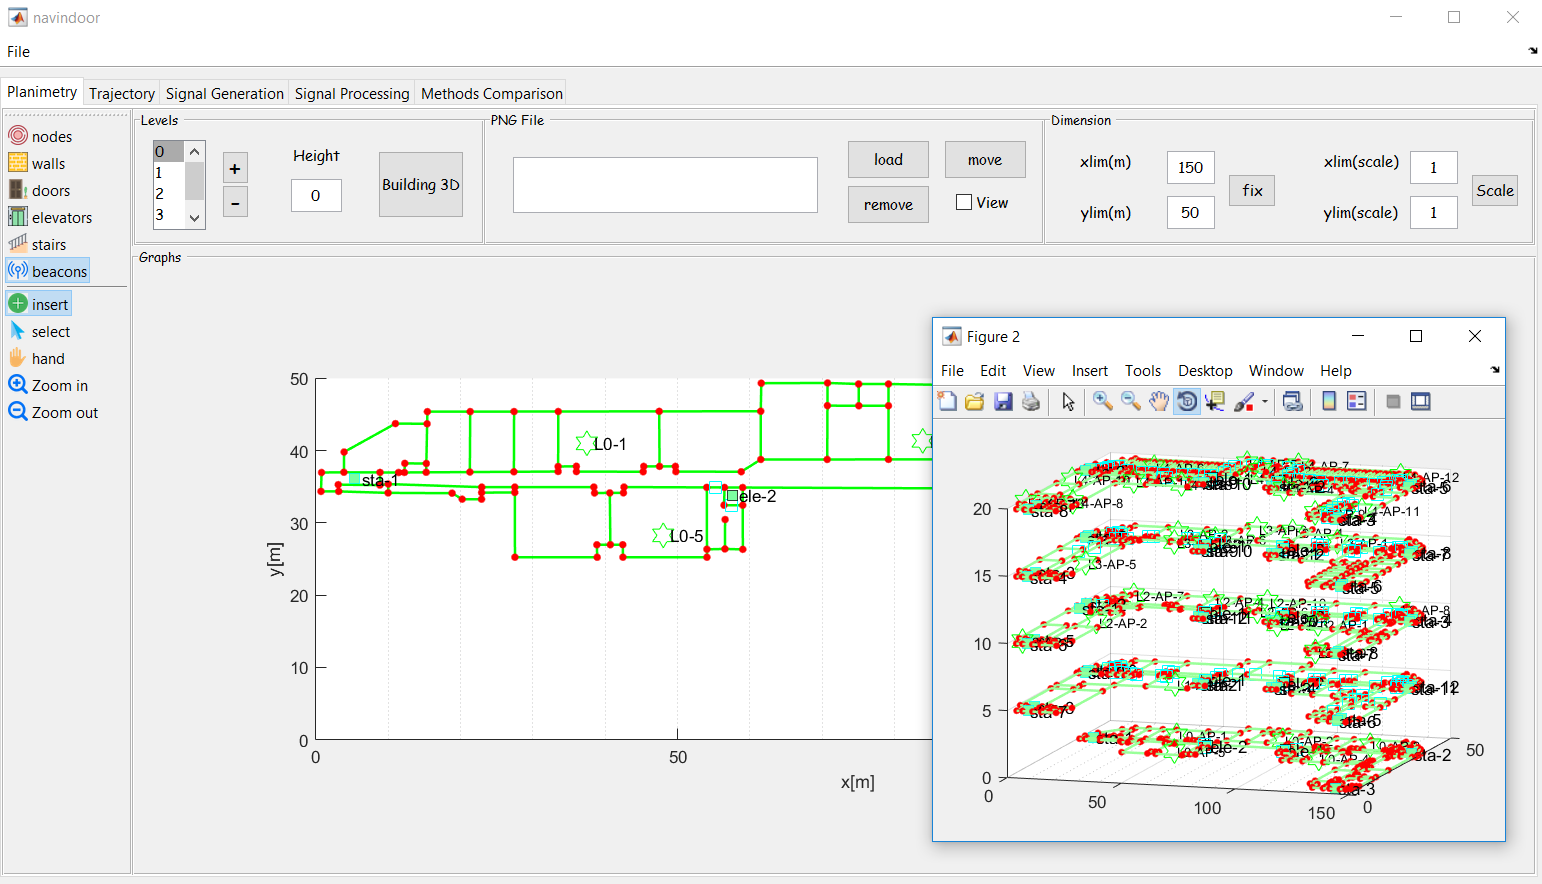
\includegraphics[width=1.05\columnwidth]{img/Design/1.PNG}
    \caption{Interfaz gráfica para el diseño de la planimetría \emph{building}.}
    \footnotesize
    En la imagen se muestra la interfaz con un edificio de cuatro plantas. La figura externa es una representación tridimensional del edificio.
    \label{fig:interfaz1}
\end{figure}

% ----------------------------------------------------------------------


